\documentclass[tikz,border=10pt]{standalone}
\usepackage{ctex}
\usepackage{xcolor}
\usetikzlibrary{shapes.arrows, positioning, calc, fit, arrows.meta}

% fig13 专属配色：硬件子系统分区 + 数据流/控制流分色
\definecolor{cNIC}{RGB}{41,98,255}     % NIC 蓝
\definecolor{cNICbg}{RGB}{232,239,255}
\definecolor{cRC}{RGB}{240,140,0}      % Root Complex 橙
\definecolor{cRCbg}{RGB}{255,246,230}
\definecolor{cPCIe}{RGB}{0,151,167}    % PCIe Controller 青
\definecolor{cPCIebg}{RGB}{224,246,248}
\definecolor{cIOMMU}{RGB}{142,68,173}  % IOMMU 紫
\definecolor{cIOMMUbg}{RGB}{244,233,250}
\definecolor{cDRAM}{RGB}{46,160,87}    % DRAM 绿
\definecolor{cDRAMbg}{RGB}{228,245,233}
\definecolor{cData}{RGB}{30,90,220}    % 数据流 蓝实线
\definecolor{cCtrl}{RGB}{220,53,53}    % 控制/背压 红虚线

\begin{document}
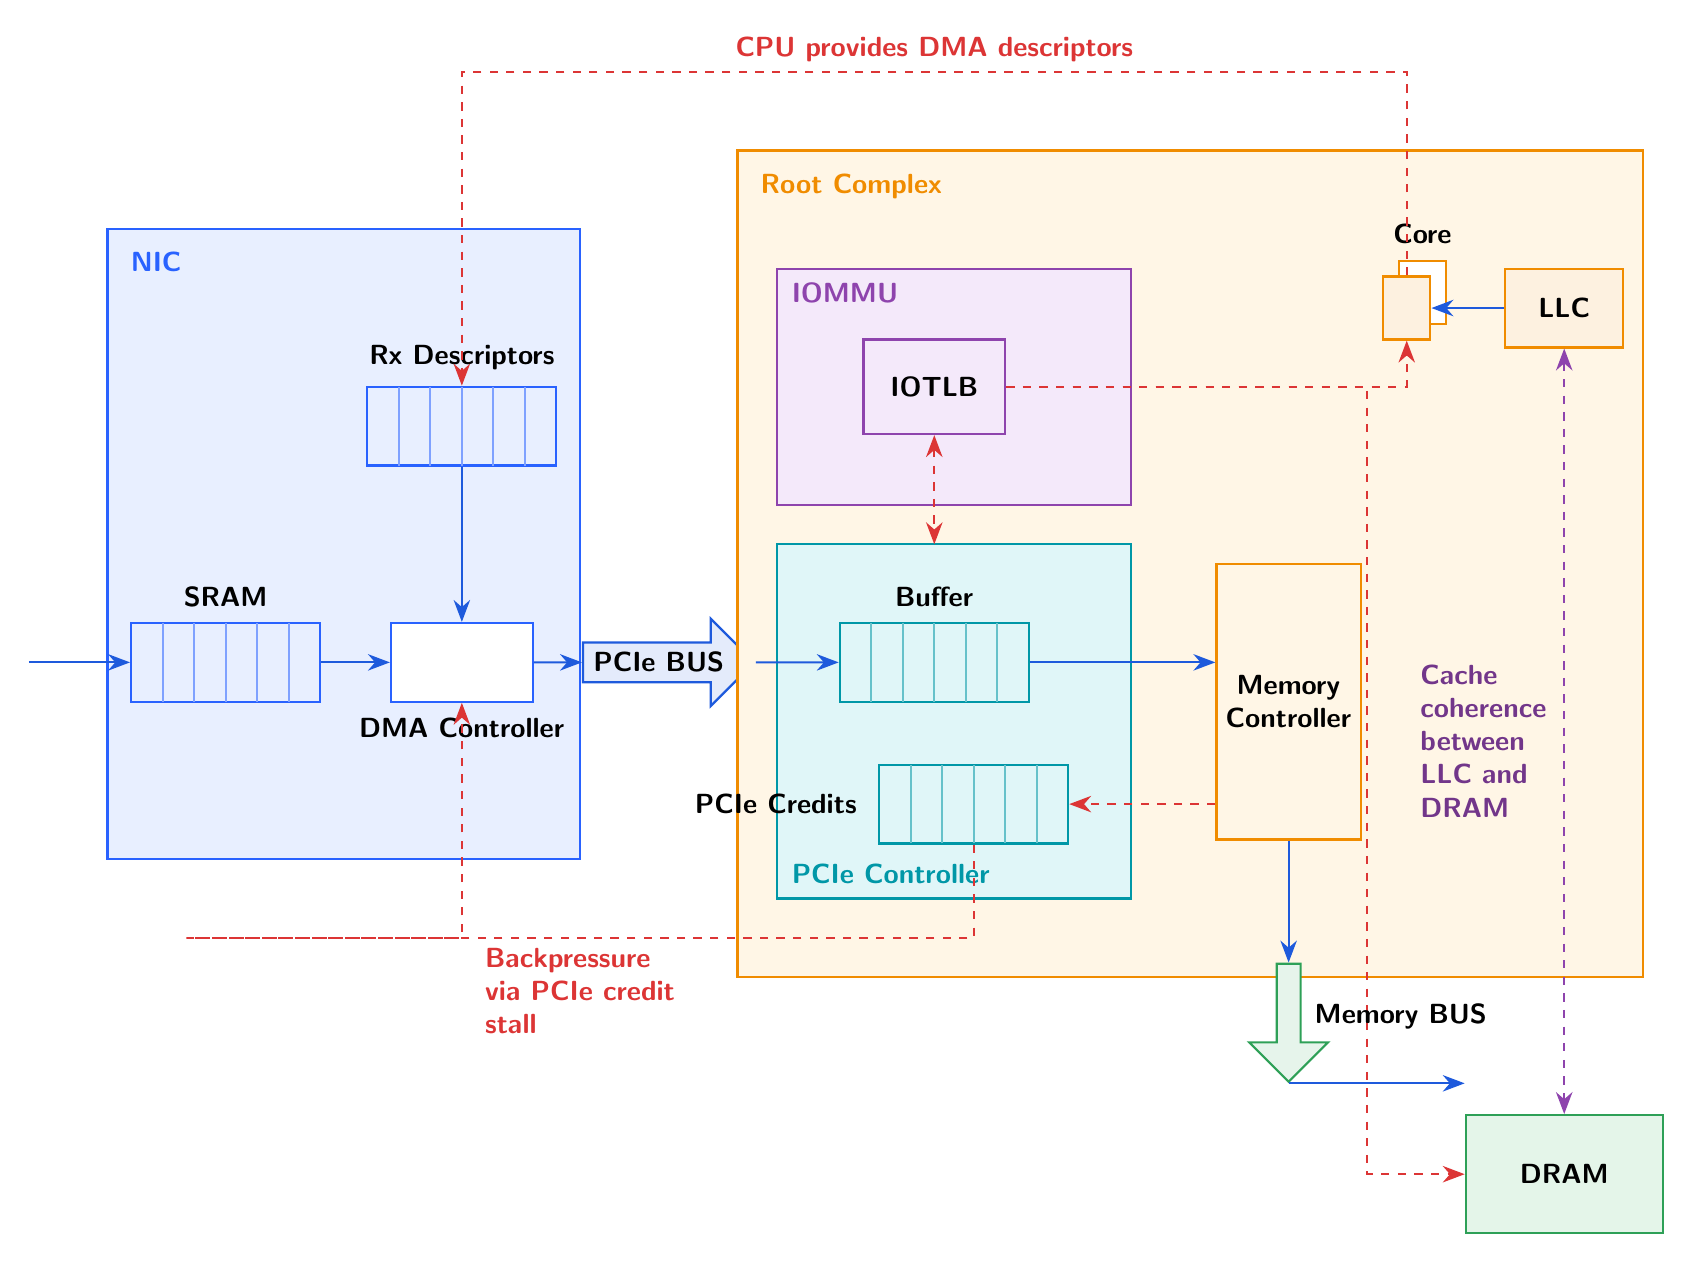
\begin{tikzpicture}[>={Stealth[scale=1.2]}, thick, font=\sffamily]

% ------------------- 定义样式 -------------------
\tikzstyle{box} = [draw=gray!70, thick, rectangle, align=center, fill=white, minimum width=1.5cm, minimum height=0.8cm]
\tikzstyle{outerbox} = [draw, thick, rectangle]
\tikzstyle{busarrow} = [draw=gray!70, thick, single arrow, fill=gray!10, minimum height=1.5cm, minimum width=1cm, single arrow head extend=3mm]
\tikzstyle{dataline} = [->, thick, cData]
\tikzstyle{ctrlline} = [->, thick, dashed, cCtrl]

% ------------------- NIC 部分 (蓝区) -------------------
\draw[outerbox, draw=cNIC, fill=cNICbg] (-1.5, -2.5) rectangle (4.5, 5.5);
\node[anchor=north west, inner sep=8pt, text=cNIC] at (-1.5, 5.5) {\textbf{NIC}};

% SRAM 队列
\node[box, fill=cNICbg, draw=cNIC, minimum width=2.4cm, minimum height=1cm, inner sep=0] (SRAM) at (0, 0) {};
\foreach \x in {-0.8,-0.4,0,0.4,0.8} \draw[thick, cNIC!60] ([xshift=\x cm]SRAM.center) ++(0,-0.5) -- ++(0,1);
\node[above=2pt of SRAM] {\textbf{SRAM}};

% Rx Descriptors 队列
\node[box, fill=cNICbg, draw=cNIC, minimum width=2.4cm, minimum height=1cm, inner sep=0] (RxQ) at (3, 3) {};
\foreach \x in {-0.8,-0.4,0,0.4,0.8} \draw[thick, cNIC!60] ([xshift=\x cm]RxQ.center) ++(0,-0.5) -- ++(0,1);
\node[above=2pt of RxQ] {\textbf{Rx Descriptors}};

% DMA Controller
\node[box, draw=cNIC, minimum width=1.8cm, minimum height=1cm] (DMA) at (3, 0) {};
\node[below=2pt of DMA] {\textbf{DMA Controller}};

% ------------------- PCIe BUS 部分 -------------------
\node[busarrow, draw=cData, fill=cData!12] (PCIeBus) at (5.5, 0) {\textbf{PCIe BUS}};

% ------------------- Root Complex 部分 (橙区) -------------------
\draw[outerbox, draw=cRC, fill=cRCbg] (6.5, -4) rectangle (18, 6.5);
\node[anchor=north west, inner sep=8pt, text=cRC] at (6.5, 6.5) {\textbf{Root Complex}};

% PCIe Controller 外框 (青)
\draw[outerbox, draw=cPCIe, fill=cPCIebg] (7, -3) rectangle (11.5, 1.5);
\node[anchor=south west, inner sep=5pt, text=cPCIe] at (7, -3) {\textbf{PCIe Controller}};

% Buffer 队列
\node[box, fill=cPCIebg, draw=cPCIe, minimum width=2.4cm, minimum height=1cm, inner sep=0] (Buffer) at (9, 0) {};
\foreach \x in {-0.8,-0.4,0,0.4,0.8} \draw[thick, cPCIe!60] ([xshift=\x cm]Buffer.center) ++(0,-0.5) -- ++(0,1);
\node[above=2pt of Buffer] {\textbf{Buffer}};

% PCIe Credits 队列
\node[box, fill=cPCIebg, draw=cPCIe, minimum width=2.4cm, minimum height=1cm, inner sep=0] (Credits) at (9.5, -1.8) {};
\foreach \x in {-0.8,-0.4,0,0.4,0.8} \draw[thick, cPCIe!60] ([xshift=\x cm]Credits.center) ++(0,-0.5) -- ++(0,1);
\node[left=4pt of Credits] {\textbf{PCIe Credits}};

% IOMMU 外框 (紫)
\draw[outerbox, draw=cIOMMU, fill=cIOMMUbg] (7, 2) rectangle (11.5, 5);
\node[anchor=north west, inner sep=5pt, text=cIOMMU] at (7, 5) {\textbf{IOMMU}};

% IOTLB
\node[box, fill=cIOMMUbg, draw=cIOMMU, minimum width=1.8cm, minimum height=1.2cm] (IOTLB) at (9, 3.5) {\textbf{IOTLB}};

% Memory Controller
\node[box, draw=cRC, fill=cRCbg, minimum width=1.5cm, minimum height=3.5cm, align=center] (MemCtrl) at (13.5, -0.5) {\textbf{Memory} \\ \textbf{Controller}};

% Core (双层框表示多个 Core)
\node[box, draw=cRC, minimum width=0.6cm, minimum height=0.8cm] (CoreBg) at (15.2, 4.7) {};
\node[box, draw=cRC, fill=cRC!12, minimum width=0.6cm, minimum height=0.8cm] (CoreFg) at (15, 4.5) {};
\node[above=2pt of CoreBg] {\textbf{Core}};

% LLC
\node[box, draw=cRC, fill=cRC!12, minimum width=1.5cm, minimum height=1cm] (LLC) at (17, 4.5) {\textbf{LLC}};

% ------------------- DRAM 部分 (绿) -------------------
\node[box, draw=cDRAM, fill=cDRAMbg, minimum width=2.5cm, minimum height=1.5cm] (DRAM) at (17, -6.5) {\textbf{DRAM}};

% ------------------- 连线与路由逻辑 -------------------

% 1. NIC 内部数据流
\draw[dataline] (-2.5, 0) -- (SRAM.west);
\draw[dataline] (SRAM.east) -- (DMA.west);
\draw[dataline] (RxQ.south) -- (DMA.north);

% 2. 跨 PCIe 数据流
\draw[dataline] (DMA.east) -- (PCIeBus.west);
\draw[dataline] (PCIeBus.east) -- (Buffer.west);

% 3. Root Complex 内部数据流
\draw[dataline] (Buffer.east) -- (MemCtrl.west |- Buffer.east);

% 4. 控制信号：CPU 提供 DMA 描述符 (最高层绕行)
\draw[ctrlline] (CoreFg.north) |- (15, 7.5) -- (3, 7.5) -- (RxQ.north);
\node[anchor=south, fill=white, text=cCtrl] at (9, 7.5) {\textbf{CPU provides DMA descriptors}};

% 5. 控制信号：IOTLB 到 Core
\draw[ctrlline] (IOTLB.east) -| (CoreFg.south);

% 6. 控制信号：IOTLB 到 PCIe Controller
\draw[<->, thick, dashed, cCtrl] (IOTLB.south) -- (9, 1.5);

% 7. 控制信号：IOTLB 到 DRAM
\draw[ctrlline] (IOTLB.east) -| (14.5, 3.5) -- (14.5, -6.5) -- (DRAM.west);

% 8. LLC 到 Core 数据流
\draw[dataline] (LLC.west) -- (CoreFg.east);

% 9. Cache Coherence (最右侧走线)
\draw[<->, thick, dashed, cIOMMU] (LLC.south) -- (DRAM.north);
\node[anchor=east, align=left, inner sep=6pt, text=cIOMMU!80!black] at (17, -1) {\textbf{Cache} \\ \textbf{coherence} \\ \textbf{between} \\ \textbf{LLC and} \\ \textbf{DRAM}};

% 10. 背压信号 (红虚线强调)
\draw[ctrlline] (MemCtrl.west |- Credits.east) -- (Credits.east);
\draw[ctrlline] (Credits.south) |- (-0.5, -3.5) -| (DMA.south);
\node[anchor=north, align=left, text=cCtrl] at (4.5, -3.5) {\textbf{Backpressure} \\ \textbf{via PCIe credit} \\ \textbf{stall}};

% 11. Memory BUS
\node[busarrow, draw=cDRAM, fill=cDRAM!12, shape border rotate=270, minimum height=1.5cm] (MemBus) at (13.5, -4.5) {};
\node[anchor=west] at (13.7, -4.5) {\textbf{Memory BUS}};
\draw[dataline] (MemCtrl.south) -- (MemBus.north);
\draw[dataline] (MemBus.south) |- (DRAM.west |- MemBus.south);

\end{tikzpicture}
\end{document}
